%03 utxos
\usetikzlibrary{calc}
%coordinate test point. Use as follows: 	\coordinate (cen) 	 	 at (0,0) (cen) [point];
\tikzset{
	every point/.style = {radius={\pgflinewidth}, opacity=1, draw, solid, fill=white},
	pt/.pic = {
		\begin{pgfonlayer}{foreground}
			\path[every point, #1] circle;
		\end{pgfonlayer}
	},
	point/.style={insert path={pic{pt={#1}}}}, point/.default={},
	point name/.style = {insert path={coordinate (#1)}}
}
%-------------------------------------------------------------------------------

%Coin Symbol--------------------------------------------------------------------
\tikzset{%
	pics/coin/.style n args={6}{%
		code ={
			\def \coinLineWidth {#1}%
			\def \coinCenDist   {#2}%
			\def \circRad       {#3}%
			\def \circColor     {#4}%
			\def \coinColorL    {#5}%
			\def \coinColor     {#6}%
			\def \signRad       {\circRad*0.20}%
			\def \signRadProp   {0.45}
			\def \signRadExt    {\signRad*\signRadProp}
			\def \signRadOut    {\signRad+\signRadExt}
			\def \signAngle     {30}
			\def \sinSignAngle  {sin(\signAngle)}
			\def \cosSignAngle  {cos(\signAngle)}
			\def \signWidth     {{pow((pow(\signRadOut,2)-pow(\sinSignAngle*\signRad,2)),0.5)-(\cosSignAngle)*\signRad)}}
			
			\def \startIX       {{cos(\signAngle)*\signRad}}
			\def \startIY       {{\sinSignAngle*\signRad}}
			
			\def \startOY       {\startIY}
			\def \signAngleOutS {{atan((\sinSignAngle*\signRad)/pow((pow(\signRadOut,2)-pow(\sinSignAngle*\signRad,2)),0.5))}}
			\def \signAngleOutE {{360-atan((\sinSignAngle*\signRad)/pow((pow(\signRadOut,2)-pow(\sinSignAngle*\signRad,2)),0.5))}}
			%
			\coordinate ()          at ( 0.0     , 0.0);%
			\coordinate (cen)       at ( 0.0     , 0.0);%
			\coordinate (cenB)      at ($(cen)    + ( 0.00,-\coinCenDist)$);%
			
			\node[
			circle,
			draw = \coinColorL,
			fill = \circColor,
			line width = \coinLineWidth,
			minimum size = \circRad,
			inner sep = 0pt,
			outer sep = 0pt,
			](NCD) at (cenB) {};
			
			\node[
			circle,
			draw = \coinColorL,
			fill = \circColor,
			line width = \coinLineWidth,
			minimum size = \circRad,
			inner sep = 0pt,
			outer sep = 0pt,
			](NCU) at (cen) {};
			
			%			\draw[ - , line width = \coinLineWidth, black] (NCU.195) -- (NCD.195);
			\draw[-, line width = \coinLineWidth, \coinColorL] (NCU.210) -- (NCD.210);
			\draw[-, line width = \coinLineWidth,\coinColorL] (NCU.225) -- (NCD.225);
			\draw[-, line width = \coinLineWidth, \coinColorL] (NCU.240) -- (NCD.240);
			\draw[-, line width = \coinLineWidth, \coinColorL] (NCU.255) -- (NCD.255);
			\draw[-, line width = \coinLineWidth, \coinColorL] (NCU.270) -- (NCD.270);
			\draw[-, line width = \coinLineWidth, \coinColorL] (NCU.285) -- (NCD.285);
			\draw[-, line width = \coinLineWidth, \coinColorL] (NCU.300) -- (NCD.300);
			\draw[-, line width = \coinLineWidth, \coinColorL] (NCU.315) -- (NCD.315);
			\draw[-, line width = \coinLineWidth, \coinColorL] (NCU.330) -- (NCD.330);
			%			\draw[ - , line width = \coinLineWidth, black] (NCU.345) -- (NCD.345);
			
			\draw[
			- ,
			line width = \coinLineWidth,
			\coinColorL,
			fill = \coinColor
			]
			(\startIX,-\startIY) arc (360-\signAngle:\signAngle:\signRad)
			-- +(\signWidth, 0.0)
			arc (\signAngleOutS:\signAngleOutE:\signRadOut)
			-- (\startIX,-\startIY)
			-- cycle
			;
		}%
		
	} ,%
	pics/coin/.default={1.0pt}{0.1}{1cm}{bg}{black!80!white}{black!90!white}%
}%
\begin{frame}{UTXO-based cryptocurrencies}
	\pgfdeclarelayer{bgutxo}
	\pgfdeclarelayer{foreground}%
	\pgfsetlayers{bgutxo,main,foreground}
	\tikz[overlay, remember picture]{%
		\only<1->{
			\begin{pgfonlayer}{bgutxo}
				\node[%
				fill      = titlebgcolor,
				anchor    = center,
				inner sep =  0pt,
				outer sep =  0pt,
				%				    xshift    = -1pt,
				]%
				at (current page.center) 
				{%
					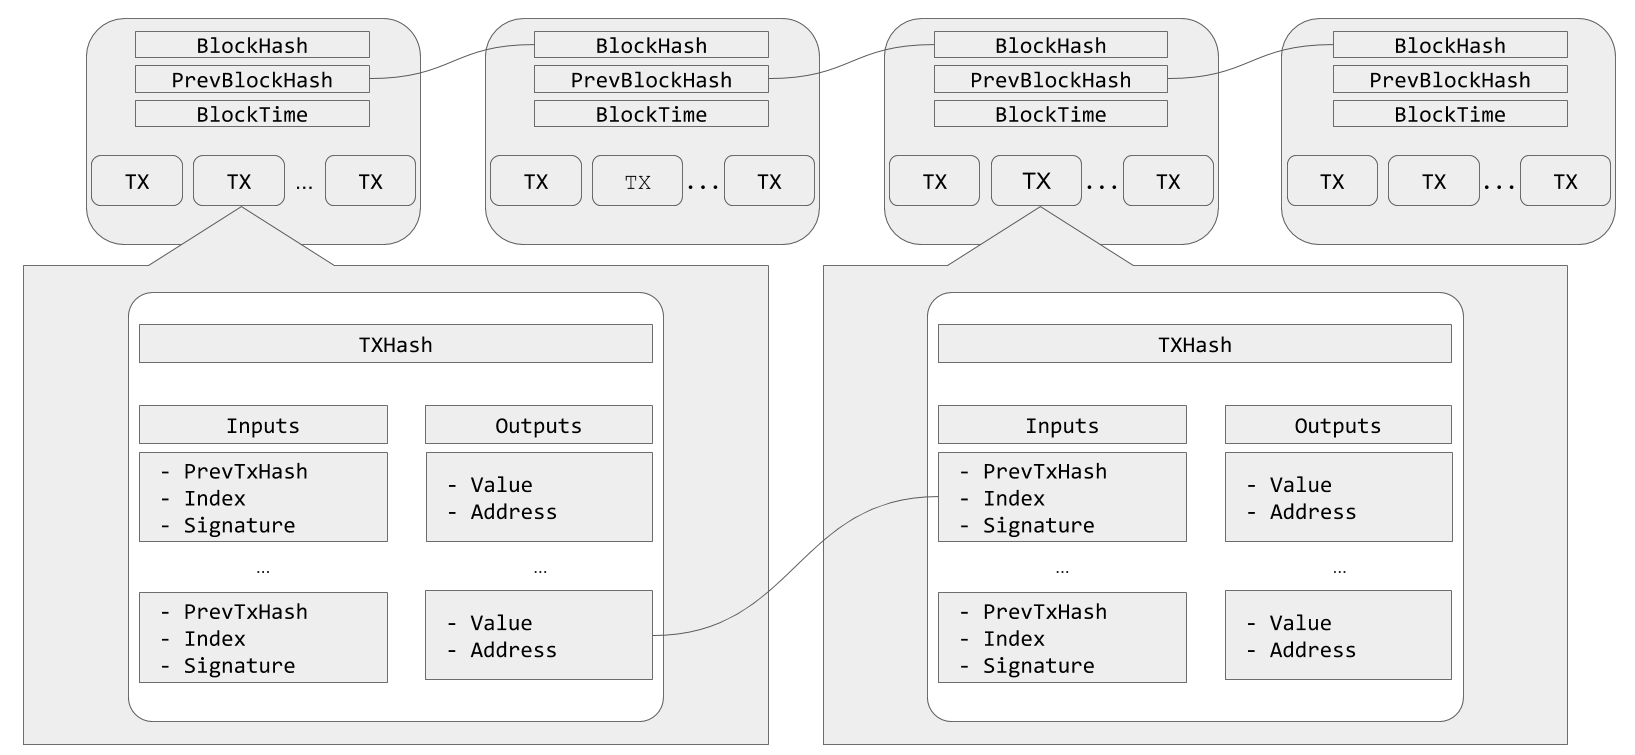
\includegraphics[scale=0.24]{./pics/used/utxo_sys_HR}%	
				};
			\end{pgfonlayer}
		}
		\only<2->{%
			\centering
			\begin{pgfonlayer}{foreground}			
				\node[fill=bg,opacity=0.75, minimum width=\linewidth, minimum height=\paperheight*0.7,inner sep=1em] at (current page.center) {};
				\inputTikz{utxoTikz}
			\end{pgfonlayer}
		}%
	}
	\vspace{1ex}
	\only<4->{%
	\begin{enumerate}\setlength{\itemsep}{1em}
		\item
			\only<4-6>{Just using \textbf{raw on-chain transaction volume} and \textbf{total coin supply} ($\VNaiveP$)}
			\only<7->{\deemphtext{Just using \textbf{raw on-chain transaction volume} and \textbf{Total coin supply}  ($\VNaiveP$)}}
		\item
			\only<4-6>{\deemphtext{Adjusting the on-chain transaction volume for \textbf{change transactions}} ($\VTotalP$)} 
			\only<7->{Adjusting the on-chain transaction volume for \textbf{change transactions} ($\VTotalP$)}
	\end{enumerate}
	}
	\vspace{30em}
\end{frame}
%-------------------------------------------------------------------------------
%\begin{frame}{UTXO-based cryptocurrencies}
%
%	\begin{figure}
%		\centering
%		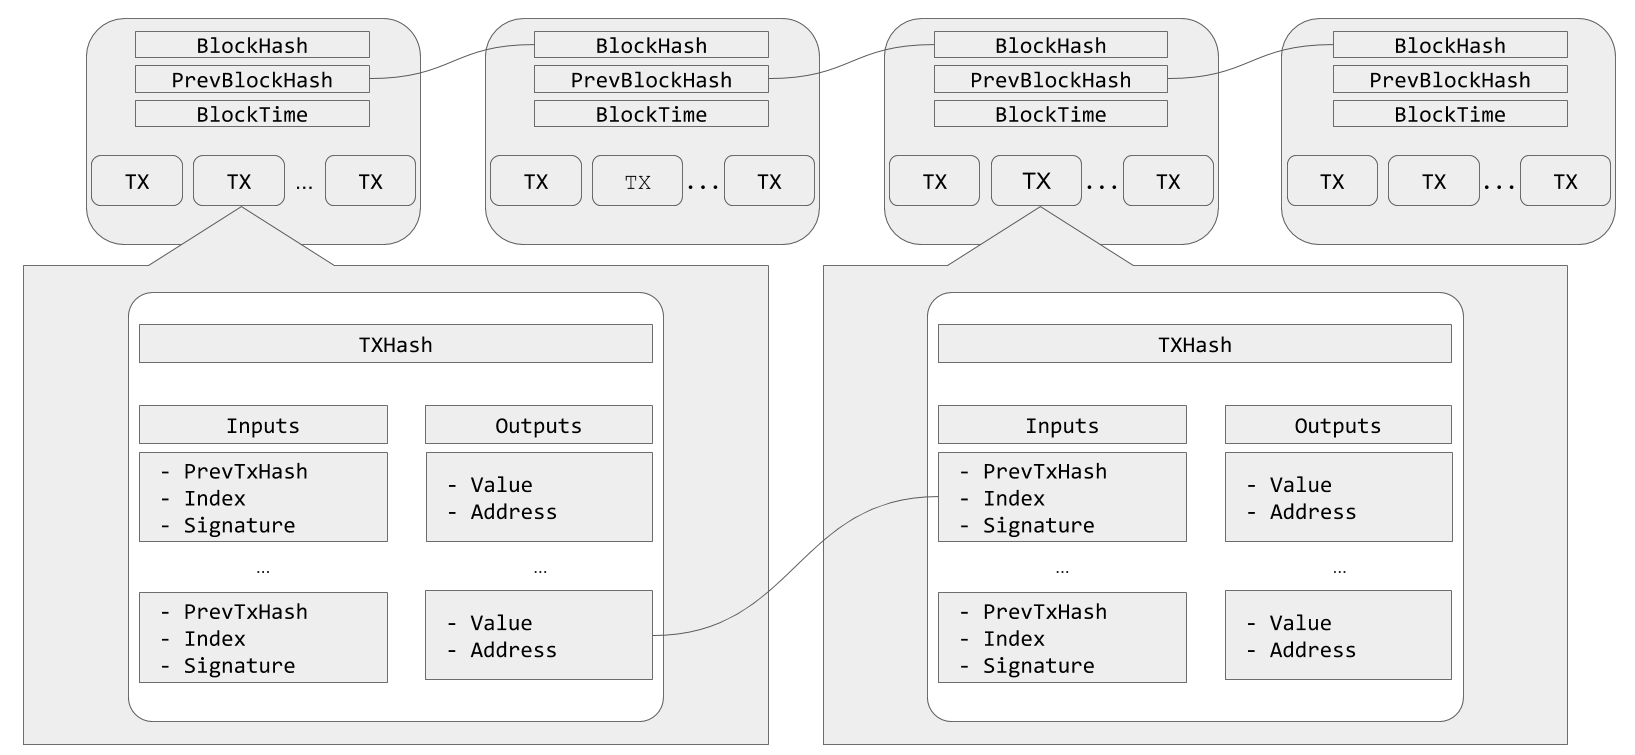
\includegraphics[scale=0.2]{./pics/used/utxo_sys_HR}
%		\caption{Blockchain and Transactions}
%	\end{figure}  
%\end{frame}

%\begin{frame}{Measuring money in effective circulation---moved coins approach}
%	\begin{figure}[h]
%		\centering
%		\inputTikz{mcirc_conceptMCA}
%		%		\caption{An example of a transaction chain.}
%	\end{figure}	
%\end{frame}